\newpage
\chapter{Dynamics}

\section{Function properties}

\subsubsection{Sine and Cosine functions}
Let a fucntion $ f(t) $ be in the form:

\begin{equation}
    f(t) = A_1 \cos{\omega t} + B_i \sin{\omega t}
\end{equation}

then the following relation applies:

\begin{eqarray}
    f(t) &= A \cos{\left( \omega t - \phi \right)}\\
    A &= \sqrt{A_1^2 + B_1^2}\\
    \phi &= \tan^{-1} \left( \frac{B_i}{A_i} \right)
\end{eqarray}

also:
\begin{eqarray}
    \cos{\left( \omega t - \phi \right)} &=
    \cos{\omega t} \cos{\phi} + \sin{\omega t} \sin{\phi}\\
    \sin{\left( \omega t - \phi \right)} &=
    \sin{\omega t} \cos{\phi} + \cos{\omega t} \sin{\phi}
\end{eqarray}



\section{SDOF system}

\subsection{Definition}

Let:

\begin{equation}
    m \ddot{u}(t) + c \dot{u}(t) + k u(t) = f(t)
\end{equation}

or:

\begin{equation}
    m a(t) + c v(t) + k u(t) = f(t)
\end{equation}

be the \textbf{SDOF equation of motion}, then the following applies:

\begin{eqarray}
    \omega^2 &= \frac{k}{m} \\
    \omega &= \sqrt{\frac{k}{m}} \\
    f &= \frac{\omega}{2 \pi} \\
    T &= \frac{1}{f}
\end{eqarray}

where:\\
$ \omega $ is radial eigenfrequency [rad/s],\\
$ f $ is eigenfrequency [Hz] and\\
$ T $ is period [s]

The simplest vibratory syslem can be described by a single mass connected to a spring
(and possibly a dashpot). The mass is allowed to travel only along the spring elongation
direction. Such systems are called \textit{Single Degree-of-Freedom} (\textbf{SDOF})
systems and are shown in the figure.

\begin{figure}[ht]
    \centering
    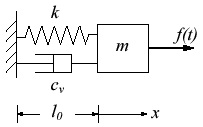
\includegraphics[width=0.90\textwidth]{img/SDOF_plot.png}
    \caption{SDOF system with a linear spring and dashpot}
    \label{fig:SDOF-plot-png}
\end{figure}


\subsection{Equation of Motion for SDOF Systems}

SDOF vibration can be analyzed by \textbf{Newton's second law of motion},
$ F = m a $. The analysis can be easily visualised with the aid of a
\textbf{free body diagram},

\begin{figure}[ht]
    \centering
    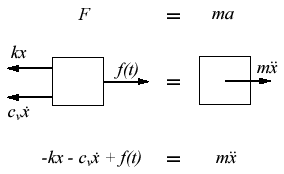
\includegraphics[width=0.90\textwidth]{img/SDOF_FreeBodyDiagram.png}
    \caption{SDOF Free Body Diagram}
    \label{fig:SDOF-freebodydiagram-png}
\end{figure}

The resulting equation of motion is a
\textbf{second order, non-homegeneous, ordinary differential equation}:

\begin{equation}
    m \ddot{u} + c \dot{u} + k u = f(t)
        \left\{ \begin{matrix}
                u(t=0) = u_0\\
                \dot{u}(t=0) = \dot{u}_0
          \end{matrix} \right.
\end{equation}

with the initial conditions $ u_0 $ and $ \dot{u}_0 $.


\subsection{Time Solution for Unforced Undamped SDOF Systems}

\textit{https://www.efunda.com/formulae/vibrations/sdof\_free\_undamped.cfm}

The equation of motion derived in the definition can be simplified to:

\begin{equation}
    m \ddot{u} + k u = 0
        \left\{ \begin{matrix}
                u(t=0) = u_0\\
                \dot{u}(t=0) = \dot{u}_0
          \end{matrix} \right.
\end{equation}

This equation of motion is a
\textbf{second order, homegeneous, ordinary differential equation} (ODE). If the mass
and spring stiffness are constants, the ODE becomes a
\textbf{linear, homogeneous ODE with constant coefficients} and can be solved
by the Characteristic Equation method. The characteristic equation for this
problem is:

\begin{equation}
    m s^2 + k = 0
\end{equation}

which determines the 2 independent roots for the undamped vibration problem.
The final solution (that contains the 2 independent roots from the characteristic
equation and satisfies the initial conditions) is:

\begin{eqarray}
    u(t) &= c_1 e^{i \omega_n t} + c_2 e^{- \omega_n t}\\
         &= d_1 \cos{\omega_n t} + d_2 \sin{\omega_n t} \\
    \implies u(t) &= u_0 \cos{\omega_n t} + \frac{\dot{u}_0}{\omega_n} \sin{\omega_n t}
\end{eqarray}

The natural frequency $ \omega_n $ is defined by:

\begin{equation}
    \omega_n = \sqrt{\frac{k}{m}}
\end{equation}

and depends only on the system mass and the spring stiffness (i.e. any damping will
not change the natural frequency of a system).

Alternatively, the solution may be expressed by the equivalent form,

\begin{equation}
    u(t) = A_0 \cos{(\omega_n t - \phi_0)}
\end{equation}

where the amplitude $ A_0 $ and the intial phase $ \phi_0 $ are given by:

\begin{eqarray}
    A_0 &= \sqrt{u_0^2 + \left(\frac{\dot{u}_0}{\omega_n}\right)^2}\\
    \phi_0 &= \tan^{-1}\frac{\dot{u}_0}{u_0 \omega_n}
\end{eqarray}

\begin{figure}[ht]
    \centering
    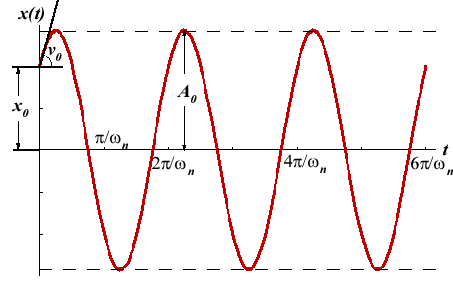
\includegraphics[width=0.90\textwidth]{img/SDOF_Undamped_Response.png}
    \caption{SDOF Undamped sample time behavior}
    \label{fig:SDOF-undamped-response-png}
\end{figure}

Note that an assumption of zero damping is typically not accurate. In reality,
there almost always exists some resistance in vibratory systems. This reistance
will damp the vibration and dissipate energy, the oscillatory motion caused by the
initial disturbance will eventually be reduced to zero.


\subsection{Time Solution for Unforced Damped SDOF Systems}

\textit{https://www.efunda.com/formulae/vibrations/sdof\_free\_damped.cfm}

\begin{figure}[ht]
    \centering
    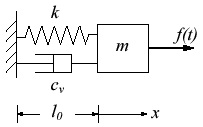
\includegraphics[width=0.90\textwidth]{img/SDOF_plot.png}
    \caption{SDOF system with a linear spring and dashpot}
    \label{fig:SDOF-plot-damped-png}
\end{figure}

Damping that produces a damping force proportional to the mass's velocity is
commonly referred to as \textit{viscous damping}, and is denoted graphically
by a dashpot.

For an unforced damped \textbf{SDOF} system, the general equation of motion
becomes:

\begin{equation}
    m \ddot{u} + c \dot{u} + k u = 0
        \left\{ \begin{matrix}
                u(t=0) = u_0\\
                \dot{u}(t=0) = \dot{u}_0
          \end{matrix} \right.
\end{equation}

Tis equation of motion is a \textbf{second order, homogeneous, ODE}. If all
parameters (mass, stiffness and viscous damping) are constants, the \textbf{ODE}
becomes a \textbf{linear ODE with constant coefficients} and can be solved by
the \textit{Characteristic Equation method}. The characteristic equation for this
problem is:

\begin{equation}
    m s^2 + s_v s + k = 0
\end{equation}

which determines the 2 independent roots for the damped vibration problem.
The roots to the characteristic equation fall into one of the following
3 cases:

\begin{itemize}
    \item If $ c_v^2 - 4 m k < 0 $, the system is termed \textbf{underdamped}.
        The roots of the characteristic equation are complex conjugates,
        corresponding to \textit{oscillatory motion} with an
        \textit{exponential decay} in amplitude.

    \item If $ c_v^2 - 4 m k = 0 $, the system is termed \textbf{critically-derdamped}.
        The roots of the characteristic equation are repeated,
        corresponding to \textit{simple decay motion} with at most
        \textit{one overshoot} of the systems resting position.

    \item If $ c_v^2 - 4 m k > 0 $, the system is termed \textbf{overderdamped}.
        The roots of the characteristic equation are prurely real and distinct,
        corresponding to \textit{simple exponentially decaying motion}.

\end{itemize}

To simplify the solutions coming up, we define the critical damping $ c_c $,
the damping ratio $ \zeta $, and the damped vibration frequency $ \omega_d $ as:

\begin{eqarray}
    c_c &= 2 m \sqrt{\frac{k}{m}} = 2 m \omega_n\\
    \zeta &= \frac{c_v}{c_c}\\
    \omega_d &= \sqrt{1 - \zeta^2} \omega_n
\end{eqarray}

where the natural frequency of the system $ \omega_n $ is given by:

\begin{equation}
    \omega_n = \sqrt{\frac{k}{m}}
\end{equation}

Note that $ \omega_d $ will equal $ \omega_n $ when the damping of the system
is zero (i.e. undamped). The time solutions for the free \textbf{SDOF}
system is presented below for each of the three case scenarios.

\subsubsection{Time Solution of Unforced Underdamped SDOF Systems}

When $ c_v^2 - 4 m k < 0 $ (equivalent to $ \zeta < 1 $ or $ c_v < c_c $),
the characteristic equation has a pair of complex conjugate roots. The displacement
solution for this kind of system is:

\begin{eqarray}
    u(t) &= c_1 e^{-\zeta + i \sqrt{1 - \zeta^2} \omega_n t}
          + c_2 e^{-\zeta - i \sqrt{1 - \zeta^2} \omega_n t}\\
         &= e^{-\zeta \omega_n t} \left[ d_1 \cos{(\omega_d t)}
                                       + d_2 \sin{(\omega_d t)} \right]\\
    \implies u(t) &= \underbrace{e^{-\zeta \omega_n t}}_{exponential\ decay}
    \underbrace{\left[ u_0 \cos{(\omega_d t)}
    + \frac{\dot{u}_0 + \zeta \omega_n u_0}{\omega_d} \sin{(\omega_d t)}
    \right]}_{periodic\ motion}
\end{eqarray}

An alternate but equivalent solution is given by:

\begin{equation}
    u(t) = A_0 \underbrace{e^{-\zeta \omega_n t}}_{exponential\ decay}
    \underbrace{\cos{(\omega_d t - \phi_0)}}_{periodic\ motion}
\end{equation}

\begin{figure}[ht]
    \centering
    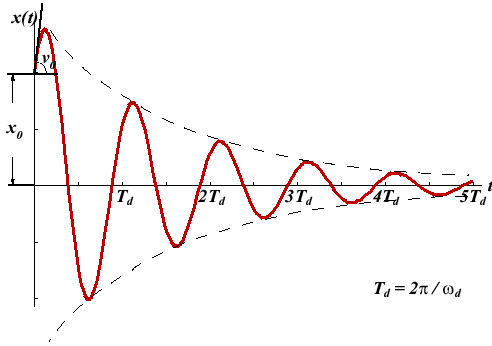
\includegraphics[width=0.70\textwidth]{img/SDOF_UnderDamped_Response.png}
    \caption{The displacement plot of an underdamped system}
    \label{fig:SDOF-underdamped-response-png}
\end{figure}

Note that the displacement amplitude decays exponentially (i.e. the natural
logarithm of the amplitude ratio for any two displacements separated in time
by a constant ratio is a constant):

\begin{eqarray}
    \frac{A_k}{A_{k+1}} &=
    \frac{A_0 e^{-\zeta \omega_n \left( k T_d \right)} \cos{ \left( \phi_0 \right) }}
         {A_0 e^{-\zeta \omega_n \left[ (k+1) T_d \right]} \cos{ \left( \phi_0 \right) }}\\
                        &=
    \frac{e^{-\zeta \omega_n \left( k T_d \right)}}
         {e^{-\zeta \omega_n \left[ (k+1) T_d \right]}}\\
                        &= e^{\zeta \omega_n T_d}\\
    \implies \ln{\left( \frac{A_k}{A_{k+1}} \right)} &=
    \zeta \omega_n T_d = \zeta \omega_n \frac{2 \pi}{\omega_d}
    = \frac{2 \pi \zeta}{\sqrt{1 - \zeta^2}}
\end{eqarray}

where $ T_d = \frac{1}{f_d} = \frac{2 \pi}{\omega_d} $ is the period of the
damped vibration.


\subsubsection{Time Solution of Unforced Critically-Damped Systems}

When $ c_v^2 - 4 m k = 0 $ (equivalent to $ \zeta = 1 $ or $ c_v = c_c $), the
characteristic equation has repeated real roots. The displacement solution for
this kind of system is:

\begin{eqarray}
    u(t) &= \left( c_1 + c_2 t \right) e^{-\omega_n t}\\
    \implies u(t) &= e^{-\omega_n t} \left[ u_0 + \left( v_0 + \omega_n u_0 \right) t \right]
\end{eqarray}

The critical damping factor $ c_c $ can be interpreted as the \textbf{minimum damping}
that results in non-periodic motion (i.e. simple decay).

\begin{figure}[ht]
    \centering
    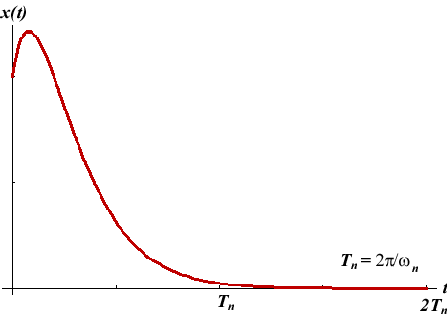
\includegraphics[width=0.70\textwidth]{img/SDOF_CriticalDamped_Response.png}
    \caption{The displacement plot of a critically-damped system with positive initial
displacement and velocity.}
    \label{fig:SDOF-critically-damped-response-png}
\end{figure}

The displacement decays to a negligible level after one natural period $ T_n $.
Note that if the initial velocity $ v_0 $ is negative while the initial displacement
$ u_0 $ is positive, there will exist one overshoot of the resting position in
the displacement plot.


\subsubsection{Time Solution of Unforced Overdamped SDOF Systems}

When $ c_v^2 - 4 m k > 0 $ (equivalent to $ \zeta > 1 $ or $ c_v > c_c $),
the characteristic equation has two distinct real roots. The displacement
solution for this kind of system is:

\begin{eqarray}
    u(t) &= c_1 e^{\left( -\zeta + \sqrt{\zeta^2 - 1} \right) \omega_n t}
          +  c_2 e^{\left( -\zeta - \sqrt{\zeta^2 - 1} \right) \omega_n t}\\
    \implies u(t) &=
    \frac{u_0 \omega_n \left( \zeta + \sqrt{\zeta^2 - 1} \right) + v_0}
    {2 \omega_n \sqrt{\zeta^2 - 1}} e^{\left( -\zeta + \sqrt{\zeta^2 - 1} \right) \omega_n t} +\\
                  &+
    \frac{-u_0 \omega_n \left( \zeta - \sqrt{\zeta^2 - 1} \right) - v_0}
    {2 \omega_n \sqrt{\zeta^2 - 1}} e^{\left( -\zeta - \sqrt{\zeta^2 - 1} \right) \omega_n t}
\end{eqarray}

\begin{figure}[ht]
    \centering
    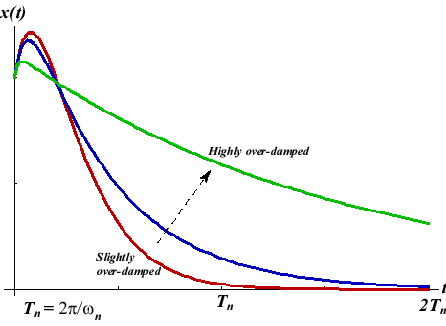
\includegraphics[width=0.70\textwidth]{img/SDOF_OverDamped_Response.png}
    \caption{The displaceent plot of an overdamped system response}
    \label{fig:SDOF-overdamped-response-png}
\end{figure}

The motion of an overdamped system is non-periodic, regardless of the inital conditions.
The larger the damping, the longer time to decay from an initial disturbance.

If the system is heavily damped, $ \zeta \gg 1 $, the displacement solution takes
the approximate form:

\begin{equation}
    u(t) \approx u_0 + \frac{v_0}{2 \zeta \omega_n}
    \left(1 - e^{-2 \zeta \omega_n t} \right)
\end{equation}


\subsection{SDOF Systems under Harmonic Excitaion}
\textit{https://www.efunda.com/formulae/vibrations/sdof\_harmo.cfm}

When a \textbf{SDOF} System is forced by $ f(t) $, the solution for the displacement
$ x(t) $ consists of two parts: the \textit{complimentary solution}, and the
\textit{particular solution}. The complimentary solution for the problem
is given by the \textbf{free vibration of an unforced SDOF System}.
The \textbf{particular solution} depends on the nature fo the forcing function.

When the forcing function is \textbf{harmonic} (i.e. it consits of at most
a \textbf{sine} and \textbf{cosine} at the same \textbf{frequency},
a quantity that can be expressed by the complex exponentional $ e^{i \omega t} $),
the method if \textbf{Undetermined Coefficients} can be used to find the particular
solution. Non-harmonic forcing functions are handled by other techniques.

Consider the SDOF system forced by the harmonic function $ f(t) $.

\begin{figure}[ht]
    \centering
    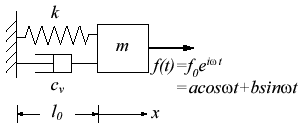
\includegraphics[width=0.70\textwidth]{img/SDOF_harmonic.png}
    \caption{SDOF System forced by the harmonic function $ f(t) $}
    \label{fig:SDOF-harmonic-response-png}
\end{figure}

The particular solution for this problem is found to be:

\begin{equation}
    u_p(t) = \frac{f_0}{ \left( k - m \omega^2 \right) + i c \omega} e^{i \omega t}
\end{equation}

The general solution is given by the sum of the complimentary and particular
solutions multiplied by two weighting constants $ c_1 $ and $ c_2 $,

\begin{equation}
    u(t) = c_1 u_c(t) + c_2 u_p(t)
\end{equation}

The values of $ c_1 $ and $ c_2 $ are found by matching $ u(t=0) $ to the
initial conditions.

\subsubsection{Undamped SDOF Systems under Harmonic Excitation}

For an undamped system ( $ c_v = 0 $ ) the total displacement solution is:

\begin{eqarray}
    u(t) &= d_1 \cos{\omega_n t} + d_2 \sin{\omega_n t} +
    \frac{f_0}{k - m \omega^2} e^{i \omega t}\\
    \implies u(t) &= \left( u_0 - \frac{f_0}{k - m \omega^2} \right) \cos{\omega_n t}\\
                  &+
    \left(\frac{v_0 - \frac{i \omega f_0}{k - m \omega^2}}{\omega_n} \right)
    \sin{\omega_n t}\\
                  &+ \frac{f_0}{k - m \omega^2} e^{i \omega t}
\end{eqarray}

If the forcing frequency is close to the natural frequency, $ \omega \approx \omega_n $,
the system will exhibit \textbf{resonance} (very large displacements) due to
near-zeros in the denominators of $ u(t) $.

When the forcing frequency is equal to the natural frequency, we cannot use the
$ u(t) $ given above as it would give divide-by-zero. Instead we must use
\textbf{L'H\^ospital's Rule} to derive a solution free of zeros in the denominators.

\begin{eqarray}
    u(t) &= u_0 \cos{\omega_n t} + \frac{v_0}{\omega_n} \sin{\omega_n t}\\
         &+ \lim_{\omega \rightarrow \omega_n} \left\{
             \frac{f_0}{k - m \omega^2} \left(
                 e^{i \omega t} - \cos{\omega_n t} - i \omega \sin{\omega_n t}
                 \right)
         \right\}\\
         &= u_0 \cos{\omega_n t} + \frac{v_0}{\omega_n} \sin{\omega_n t}
         - \frac{f_0 \omega_n}{2 k} \left(
             i t e^{i \omega)n t} - i \sin{\omega_n t}
             \right)
\end{eqarray}

To simplify $ u(t) $, let's assume that the driving force consists only of the
cosine function $ f(t) = f_0 \cos{\omega t} $.

\begin{figure}[ht]
    \centering
    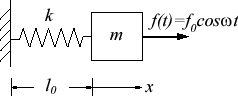
\includegraphics[width=0.35\textwidth]{img/SDOF_harmonic_undamped.png}
    \caption{SDOF System forced by the harmonic function $ f(t) = f_0 \cos{\omega t} $}
    \label{fig:SDOF-harmonic-undamped-response-png}
\end{figure}

The displacement solution reduces to:

\begin{eqarray}
    u(t) &= u_0 \cos{\omega_n t} + \frac{v_0}{\omega_n} \sin{\omega_n t}\\
         &+ \lim_{\omega \rightarrow \omega_n} \left\{
             \frac{f_0}{k - m \omega^2} \left(
                 \cos{\omega t} - \cos{\omega_n t}
                 \right)
         \right\}\\
         &= \underbrace{u_0 \cos{\omega_n t} + \frac{v_0}{\omega_n} \sin{\omega_n t}}_{
         free\ vibration\ (complementary)}
         + \underbrace{\frac{f_0 \omega_n t}{2 k}}_{\Scale[0.75]{
             \begin{matrix}
                 amplitude\\
                 linearly\\
                 increased
             \end{matrix}}}
         \sin{\omega_n t}
\end{eqarray}

This solution contains one term multiplied by $ t $. This term will cause the displacement
amplitude to increase linearly wit time as the forcing function pumps energy into
the system.

\begin{figure}[ht]
    \centering
    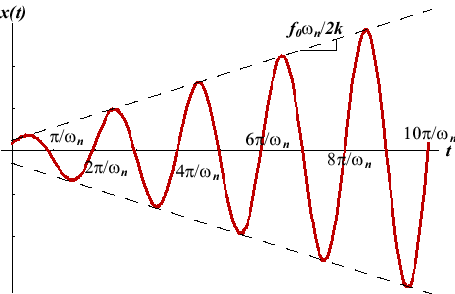
\includegraphics[width=0.70\textwidth]{img/SDOF_Undamped_Harmonic_Response.png}
    \caption{Resonance response of undamped SDOF with harmonic excitation}
    \label{fig:SDOF-undamped-harmonic-response-png}
\end{figure}

The maximum displacement of an undamped system forced at its resonant frequency will
increase unbounded according to the solution for $ u(t) $ above. However, real systems
will inject additional physics once displacements become large enough. These
additional physics (nonlinear plastic deformation, heat transfer, buckling etc.) will
serve to limit the maximum displacement exhibited by the system, and allow one to escape
the "sudden death" impression that such systems will immediately fail.


\subsubsection{Damped SDOF Systems under Harmonic Excitation}

\begin{equation}
    m \ddot{u} + c \dot{u} + k u = F_0 \cos{\left(\omega t \right)}
\end{equation}

then \textbf{steady state} solution is in the form:

\begin{equation}
    u_{s.s.} = u_0 \cos{\left(\omega t - \phi \right)}
\end{equation}

If we plug the \textbf{steady state} solution to the \textbf{equation of motion},
we get:

\begin{eqarray}
    u_o \left[ \left(k - m \omega^2\right) \cos{\omega t - \phi} -
    c \omega \sin{\left( \omega t - \phi \right)} \right]
    &= F_0 \cos{\left( \omega t \right)} \quad \vert \times \frac{1}{k}\\
        u_o \left[ \left(1 - \frac{\omega^2}{\omega_n^2} \right) \cos{\omega t - \phi} -
        2 \zeta \frac{\omega}{\omega_n} \sin{\left( \omega t - \phi \right)} \right]
    &= \frac{F_0}{k} \cos{\left( \omega t \right)}
\end{eqarray}

because:
\begin{equation}
    \frac{k}{m} = \omega_n
\end{equation}

\begin{equation}
    \zeta = \frac{c}{c_c}
\end{equation}

\begin{equation}
    c = 2 m \sqrt{\frac{k}{m}} = 2 m \omega_n
\end{equation}

\begin{equation}
    \frac{c}{k} = \frac{\zeta c_c}{k} = \frac{\zeta 2 m \omega_n}{k}
    = \frac{2 \zeta \omega_n^2}{omega_n^2} = \frac{2 \zeta}{\omega_n}
\end{equation}

after utilising the sine and cosine relations:

\begin{eqarray}
    \cos{\left( \omega t - \phi \right)} &=
    \cos{\omega t} \cos{\phi} + \sin{\omega t} \sin{\phi}\\
    \sin{\left( \omega t - \phi \right)} &=
    \sin{\omega t} \cos{\phi} + \cos{\omega t} \sin{\phi}
\end{eqarray}

we get a set of two equatons:
\begin{eqarray}
    u_o \left[ \left(1 - \frac{\omega^2}{\omega_n^2} \right) \cos{\phi} +
    2 \zeta \frac{\omega}{\omega_n} \sin{\phi} \right] \cos{\omega t}
    &= \frac{F_0}{k} \cos{\left( \omega t \right)}\\
    u_o \left[ \left(1 - \frac{\omega^2}{\omega_n^2} \right) \sin{\phi} -
    2 \zeta \frac{\omega}{\omega_n} \cos{\phi} \right] \sin{\omega t}
    &= 0\\
\end{eqarray}

and when solving just for amplitudes this reduces to a set of two algebraic equations
which is then solved for $ u_0 $ and $ \phi $:
\begin{eqarray}
    u_o \left[ \left(1 - \frac{\omega^2}{\omega_n^2} \right) \cos{\phi} +
    2 \zeta \frac{\omega}{\omega_n} \sin{\phi} \right]
    &= \frac{F_0}{k}\\
    u_o \left[ \left(1 - \frac{\omega^2}{\omega_n^2} \right) \sin{\phi} -
    2 \zeta \frac{\omega}{\omega_n} \cos{\phi} \right]
    &= 0\\
\end{eqarray}

The solution (\textbf{transfer function}) is finally:
\begin{eqarray}
    u_0 &= \frac{\frac{F_0}{k}}{
        \left[
            \left( 1 - \frac{\omega^2}{\omega_n^2} \right)^2 +
            \left( 2 \zeta \frac{\omega}{\omega_n} \right)^2
    \right]^{\frac{1}{2}}}\\
    \phi &= \tan^{-1} \left(
        \frac{2 \zeta \frac{\omega}{\omega_n}}{
    1 - \frac{\omega^2}{\omega_n^2}} \right)
\end{eqarray}

where:\\
$ u_0 $ is displacement amplitude\\
$ \frac{F_0}{k} $ is displacement from static simulation.

\begin{equation}
    H_0 = \frac{\frac{F_0}{k}}{
        \left[
            \left( 1 - \frac{\omega^2}{\omega_n^2} \right)^2 +
            \left( 2 \zeta \frac{\omega}{\omega_n} \right)^2
    \right]^{\frac{1}{2}}}
\end{equation}





\newpage
\section{Damping}

\subsection{Rayleigh Damping}
\textit{https://www.simscale.com/knowledge-base/rayleigh-damping-coefficients/}

Let \textbf{Rayleigh Damping} be defined as:

\begin{equation}
    c = \alpha k + \beta m
\end{equation}

where:\\
$ c $ is damping value [-],\\
$ \alpha $ is stiffness dependent damping coefficient,\\
$ \beta $ is inertia (mass) dependent damping coefficient,\\
$ m $ is mass and\\
$ k $ is stiffness.

Thus, substituting this relation to the equation of motion:

\begin{eqarray}
    m \ddot(u) + \left(\alpha k + \beta m \right) \dot{u} + k u &= f(t) & \space \vert \times \frac{1}{m}\\
    \ddot{u} + \left(\alpha \frac{k}{m} + \beta \frac{m}{m} \right) \dot{u} + \frac{k}{m} u
    &= \frac{f(t)}{m} & \space \vert \frac{k}{m} = \omega_n^2 \\
    \ddot{u} + \left(\alpha \omega_n^2 + \beta \right) \dot{u} + \omega_n^2 u &= \frac{f(t)}{m} & \space
\end{eqarray}

Damping Ratio:

\begin{eqarray}
    \zeta &= \frac{c}{2 m \omega_n}\\
    \zeta &= \frac{1}{2 m \omega_n} \left( \alpha k + \beta m \right)\\
    \zeta &= \frac{1}{2} \left( \alpha \omega_n + \frac{\beta}{\omega_n} \right)
\end{eqarray}

where:\\
$ \zeta $ is damping ratio,\\
$ c $ is damping value [-],\\
$ m $ is mass and\\
$ \omega_n $ is natural frequency [rad/s]

Substituting back:

\begin{equation}
    \ddot{u} + 2 \zeta \omega_n \dot{u} + \omega_n^2 k u = \frac{f(t)}{m}
\end{equation}


When \textbf{Damping is proportional to inertia}:

In this case, the stiffness coefficient $ \alpha = 0 $ and thus:

\begin{equation}
    \zeta = \frac{\beta}{2 \omega_n}
\end{equation}

For a given constant value of $ \beta $, it is seen that the damping is inversely
proportional to the natural frequency, as shown in the illustration:

\begin{figure}[ht]
    \centering
    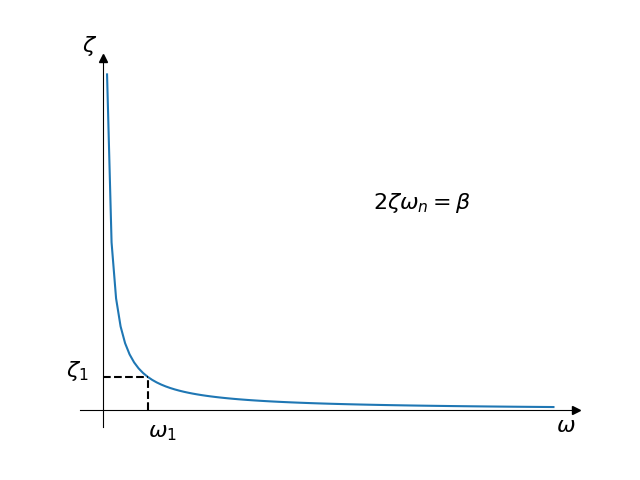
\includegraphics[width=0.90\textwidth]{img/inertia_dependent_damping.png}
    \caption{Schematic of damping proportional to inertia}
    \label{fig:inertia-dependent-damping-png}
\end{figure}

Moreover, if one computes $ \beta $ from the damping ration $ \zeta_1 $ at a given
natural frequency $ \omega_1 $, all the natural frequencies below it will be amplified
and the frequencies above it will be attenuated. The effect is more dramatic the farther
the frequencies are from the reference value.

When \textbf{Damping is proportional to stiffness}:

In this case, the mass coefficient $ \beta = 0 $ and thus:

\begin{equation}
    \zeta = \frac{1}{2} \alpha \omega_n
\end{equation}

It is seen that, contrary to the first case, here the damping id directly proportional
to the natural frequency:

\begin{figure}[ht]
    \centering
    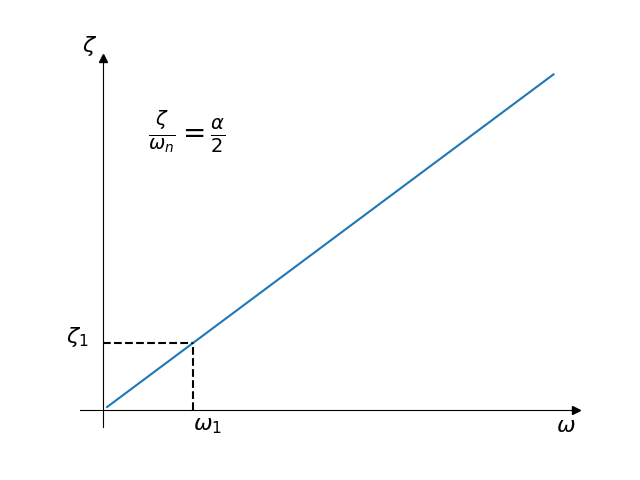
\includegraphics[width=0.90\textwidth]{img/stiffness_dependent_damping.png}
    \caption{Schematic of damping proportional to stiffness}
    \label{fig:stiffness-dependent-damping-png}
\end{figure}

If one computes $ \alpha $ from the damping ratio $ \zeta_1 $ at a natural
frequency $ \omega_1 $, then the natural frequencies below will be attenuated and
the frequencies above will be amplified.

\textbf{General Case}:

In the case of using the model with two parameters, the proportionality of damping
against frequency is convex:

\begin{figure}[ht]
    \centering
    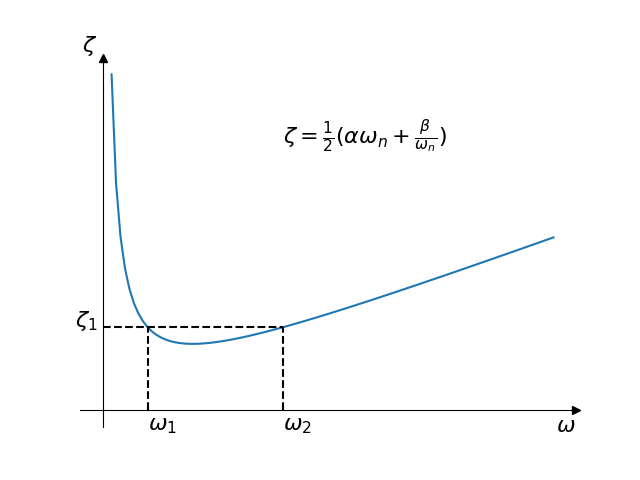
\includegraphics[width=0.90\textwidth]{img/general_rayleigh_damping.png}
    \caption{Schematic of full damping model}
    \label{fig:general-rayleigh-damping-png}
\end{figure}

In this case one needs two damping ratios and two natural frequencies to create
a pair of equations and solve for $ \alpha $ and $ \beta $. The model gives some
flexibility on where to place the natural frequencies, but in general, frequencies
too far away from the ones used in the computation will be amplified.

In the particular case of using equal damping ratios for the two frequencies,
it is important to note that the damping ratio \textbf{will not be constant inside the range}
defined by the sample points, but the inner frequencies will be attenuated. That is,
the inner frequencies will have a lower damping ratio.

\textbf{Computing the Rayleigh Damping Coefficients}

In the most common case, a transient response curve frim the system is obtained and
the damping ratio $ \zeta_1 $ is determined for the lowest natural frequency
$ \omega_1 $ by measuring the (logarithmic) attenuation of successive peaks.

\begin{figure}[ht]
    \centering
    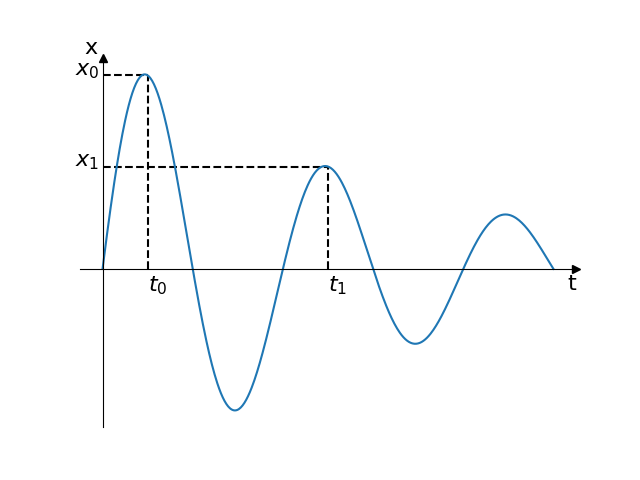
\includegraphics[width=0.90\textwidth]{img/Logarithmic_Decay_Damping_Ratio.png}
    \caption{Determination of the damping ration from the logarithmic decay}
    \label{fig:logarithmic-decay-damping-ratio-png}
\end{figure}

\begin{eqarray}
    \zeta &= \frac{\delta}{\sqrt{\delta^2 + (2 \pi)^2}}\\
    \delta &= \ln{\frac{x_0}{x_1}}\\
    f &= \frac{1}{T} = \frac{1}{t_1 - t_0}\\
    \omega &= 2 \pi f
\end{eqarray}

It is then most common to assume the case of damping proportional to the stiffness,
that is, $ \beta = 0 $, and the $ \alpha $ stiffness coefficient is computed from:

\begin{equation}
    \alpha = \frac{2 \zeta_1}{\omega_1} = \frac{\zeta+1}{\pi f_1}
\end{equation}

If the knowledge on the system indicates the case of damping decreasing with the
frequency, then one can assume the case of damping proportional to the inertia,
where $ \alpha = 0 $ and determine the mass coefficient $ \beta $:

\begin{equation}
    \beta = 2 \zeta_1 \omega_1 = 4 \pi \zeta_1 f_1
\end{equation}

If there is not such test data or knowledge of the system, or if one wishes to apply
an approximate damping ration over a range of frequencies, then we can use the
general case and build a system of two equations:

\begin{eqarray}
    \zeta_1 &= \frac{1}{2} \left( \alpha \omega_1 + \frac{\beta}{\omega_1} \right)\\
    \zeta_2 &= \frac{1}{2} \left( \alpha \omega_2 + \frac{\beta}{\omega_2} \right)
\end{eqarray}

Then solve for the unknown coefficients, keeping in mint the considerations given
above for the general case and the influence of the model on natural frequencies
inside and outside the range of interest. That is, perhaps one wants to achieve
a mean damping ratio over the range, then compensate the attenuation by modifying
the input damping rations, or by performing some least-squares approximation from
more than two frequency points.







\newpage
\section{Modal decomposition}

\subsection{Definition}

Let:

\begin{equation}
    \m{M}\ddot{\m{u}} + \m{C}\dot{\m{u}} +  \m{K}\m{u} = \m{F}\left( t \right)
\end{equation}

be the \textbf{equation of motion}, then:\\
$ \M{\Lambda} $ is a \textbf{spectral} matrix\\
$ \M{\Psi} $ is a \textbf{mode shape} matrix,

such that:
\begin{equation}
    \M{\Lambda} =
    \begin{bmatrix}
        \lambda_1^2 & \dots & 0\\
        \vdots & \ddots & \vdots \\
        0 & \dots & \lambda_n^2
    \end{bmatrix}
\end{equation}

where $ \lambda_n^2 $ is the n-th eigenvalue of the problem
$ (\m{K}-\lambda^2\m{M})\m{X} = 0 $

and:
\begin{equation}
    \M{\Psi} =
    \begin{bmatrix}
        \M{\psi}_1 & \dots & \M{\psi}_n
    \end{bmatrix}
\end{equation}

where $ \M{\psi}_n = \{\psi_{n,1}, \dots, \psi_{n,m}\}^T $ is the eigenvector
of the n-th eigenvalue $ \lambda_n^2 $.

The \textbf{displacement} $ \m{u} $ can be expressed as a linear combination
of eigenvectors such that:

\begin{eqarray}
    \m{u}(t)
    &= \M{\Psi} \m{q}(t) \\
    &= \begin{bmatrix}
        \M{\psi}_1 & \dots & \M{\psi}_n
    \end{bmatrix} \m{q}(t) \\
    &= \begin{bmatrix}
        \M{\psi}_{1,1} & \dots & \M{\psi}_{n,1} \\
        \vdots & \vdots & \vdots \\
        \M{\psi}_{1,m} & \dots & \M{\psi}_{n,m}
    \end{bmatrix}
    \begin{bmatrix}
        q_1(t) \\
        \vdots \\
        q_n(t)
    \end{bmatrix}
\end{eqarray}

where $ \m{q}(t) $ is a vector of modal coefficients.

Then:

\begin{eqarray}
    \dot{\m{u}}(t) &= \M{\Psi} \dot{\m{q}}(t) \\
    \ddot{\m{u}}(t) &= \M{\Psi} \ddot{\m{q}}(t)
\end{eqarray}

First we substitute $ \m{u} = \M{\Psi}\m{q} $ to the
\textbf{equation of motion}:

\begin{equation}
    \m{M} \M{\Psi} \ddot{q} +
    \m{C} \M{\Psi} \dot{q} +
    \m{K}\M{\Psi}\m{q}
    = \m{F}(t)
\end{equation}

By \textbf{premultiplying} with $ \M{\Psi}^T $ we get:

\begin{equation}
    \M{\Psi}^T \m{M} \M{\Psi} \ddot{\m{q}} +
    \M{\Psi}^T \m{C} \M{\Psi} \dot{\m{q}} +
    \M{\Psi}^T \m{K} \M{\Psi} \m{q} =
    \M{\Psi}\m{F}(t) = \m{Q}(t)
\end{equation}

where $ \m{Q}(t) = \M{\Psi} \m{F}(t) $ is called a \textbf{modal load}.

\subsection{Orthonormalised Modal Base}

Then one can exploit the properties of \textbf{orthonormalised eigenvectors}, where:

\begin{equation}
    \M{\psi}_r^T \M{\psi}_s = 0 \Leftrightarrow r \neq s
\end{equation}

The \textbf{mass}, \textbf{damping} and \textbf{stiffness} matrices are therefore
reduced to:

\begin{eqarray}
    \M{\Psi}^T \m{M} \M{\Psi}
    &= \begin{bmatrix}
        m_1 & \dots & 0 \\
        \vdots & \ddots & \vdots \\
        0 & \dots & m_n
    \end{bmatrix} \\
    \M{\Psi}^T \m{C} \M{\Psi}
    &= \begin{bmatrix}
        c_1 & \dots & 0 \\
        \vdots & \ddots & \vdots \\
        0 & \dots & c_n
    \end{bmatrix} \\
    \M{\Psi}^T \m{K} \M{\Psi}
    &= \begin{bmatrix}
        k_1 & \dots & 0 \\
        \vdots & \ddots & \vdots \\
        0 & \dots & k_n
    \end{bmatrix}
\end{eqarray}

where: \\
$ m_i $ is the \textbf{modal mass} of the i-th shape\\
$ c_i $ is the \textbf{modal damping} of the i-th shape\\
$ k_i $ is the \textbf{modal stiffness} of the i-th shape

\begin{bbox}[0.96]
    \textbf{Note}:

    When are the eigenvectors \textbf{orthonormalised} to \textbf{mass}, the above
    equations reduce to:

    \begin{eqarray}
        \M{\Psi}^T \m{M} \M{\Psi}
        &= \begin{bmatrix}
            1.0 & \dots & 0 \\
            \vdots & \ddots & \vdots \\
            0 & \dots & 1.0
        \end{bmatrix} = \m{I} \\
        \M{\Psi}^T \m{C} \M{\Psi}
        &= \begin{bmatrix}
            c_1 & \dots & 0 \\
            \vdots & \ddots & \vdots \\
            0 & \dots & c_n
        \end{bmatrix} \\
        \M{\Psi}^T \m{K} \M{\Psi}
        &= \begin{bmatrix}
            \lambda_1^2 & \dots & 0 \\
            \vdots & \ddots & \vdots \\
            0 & \dots & \lambda_n^2
        \end{bmatrix} = \M{\Lambda}^2
    \end{eqarray}

    \textbf{Mass normalisation}:

    \begin{equation}
        \M{\psi}_{i,mass} = \frac{\M{\psi}_i}{\M{\psi}_i^T \m{m}_i \M{\psi}_i}
    \end{equation}

    where:

    $ \m{m}_i $ is the i-th row of the \textbf{mass} matrix $ \m{M} $.

\end{bbox}


\subsection{MDOF to SDOF}

The MDOF \textbf{equation of motion} can be then rewritten as a set of \textbf{SDOF}
equations:

\begin{eqarray}
    \M{\Psi}^T \m{M} \M{\Psi} \ddot{\m{q}}(t) +
    \M{\Psi}^T \m{C} \M{\Psi} \dot{\m{q}}(t) +
    \M{\Psi}^T \m{K} \M{\Psi} \m{q}(t) &=
    \M{\Psi}^T \m{F}(t) \\
    \m{M}_{\Psi} \ddot{\m{q}}(t) +
    \m{C}_{\Psi} \dot{\m{q}}(t) +
    \m{K}_{\Psi} \m{q}(t) &= \m{Q}(t)
\end{eqarray}

Written explicitely:

\begin{eqarray}
    \begin{bmatrix}
        m_1 & \dots & 0 \\
        \vdots & \ddots & \vdots \\
        0 & \dots & m_n
    \end{bmatrix}
    \begin{bmatrix}
        \ddot{q}_1(t) \\
        \vdots \\
        \ddot{q}_n(t)
    \end{bmatrix} &+ \\
    \begin{bmatrix}
        c_1 & \dots & 0 \\
        \vdots & \ddots & \vdots \\
        0 & \dots & c_n
    \end{bmatrix}
    \begin{bmatrix}
        \dot{q}_1(t) \\
        \vdots \\
        \dot{q}_n(t)
    \end{bmatrix} &+ \\
    \begin{bmatrix}
        k_1 & \dots & 0 \\
        \vdots & \ddots & \vdots \\
        0 & \dots & k_n
    \end{bmatrix}
    \begin{bmatrix}
        q_1(t) \\
        \vdots \\
        q_n(t)
    \end{bmatrix} &=
    \begin{bmatrix}
        Q_1(t) \\
        \vdots \\
        Q_n(t)
    \end{bmatrix}
\end{eqarray}

It is important to note that all modal matrices (mass, damping and stiffness) are
purely diagonal (with simple enough damping), so the \textbf{MDOF} problem reduces to a series
of \textbf{SDOF} problems:

\begin{eqarray}
    m_1 \ddot{q}_1(t) + c_1 \dot{q}_1(t) + k_1 q_1(t) &= Q_1(t) \\
    m_2 \ddot{q}_2(t) + c_2 \dot{q}_2(t) + k_2 q_2(t) &= Q_2(t) \\
    \vdots \\
    m_n \ddot{q}_n(t) + c_n \dot{q}_n(t) + k_n q_n(t) &= Q_n(t)
\end{eqarray}

which are solved separately and the results are \textbf{linearly} combined:

\begin{eqarray}
    \m{u} = \sum_{i=1}^n \M{\psi}_i q_i \\
    \m{\dot{u}} = \sum_{i=1}^n \M{\psi}_i \dot{q}_i \\
    \m{\ddot{u}} = \sum_{i=1}^n \M{\psi}_i \ddot{q}_i
\end{eqarray}

\begin{bbox}[0.96]
    \textbf{Note:} Above equation can be also written as:

    \begin{eqarray}
        \m{u} = \sum_{i=1}^n \M{\psi}_i q_{u,i} \\
        \m{v} = \sum_{i=1}^n \M{\psi}_i q_{v,i} \\
        \m{a} = \sum_{i=1}^n \M{\psi}_i q_{a,i}
    \end{eqarray}

    where:\\
    $ \m{u} $ is displacement \\
    $ \m{v} $ is velocity \\
    $ \m{a} $ is acceleration

    and\\
    $ \m{q}_{u} $ is modal displacement \\
    $ \m{q}_v $ is modal velocity \\
    $ \m{q}_a $ is modal acceleration

\end{bbox}


\subsection{Initial Conditions}

To get the initial modal conditions, one simply:

\begin{eqarray}
    \m{q}_0 &= \M{\Psi}^{-1} \m{u}_0 \\
    \m{\dot{q}}_0 &= \M{\Psi}^{-1} \m{\dot{u}}_0 \\
    \m{\ddot{q}}_0 &= \M{\Psi}^{-1} \m{\ddot{u}}_0
\end{eqarray}

where:\\
$ \M{\Psi}^{-1} $ is an inverse of eigenshape matrix $ \Leftrightarrow $ all eigenvalues
and eigenshapes are used.

\begin{bbox}[0.96]
    \textbf{Note}: This is not usually so. Normally one would use
    \textbf{reduced modal base}, where only the first \textbf{n} eigenmodes are used. Then
    $ \M{\Psi}^{-1} $ is written as $ \M{\Psi}^{+} $ and called the
    \textbf{pseudoinverse of mode shape matrix} defined (at least in \textbf{numpy}
    - \textit{numpy.linal.pinv()}) as:\\

    \smallskip
    The pseudo-inverse of a matrix $ \m{A} $, denoted $ \m{A}^{+} $,
    is defined as: “the matrix that ‘solves’ [the least-squares problem]
    $ \m{A} \m{x} = \m{b} $ ,” i.e., if $ \overline{\m{x}} $
    is said solution, then $ \m{A}^{+} $ is that matrix such that
    $ \overline{\m{x}} = \m{A}^{+} \m{b} $.\\

    \smallskip
    It can be shown that if $ \m{Q}_1 \M{\Sigma} \m{Q}_2^T = \m{A} $
    is the singular value decomposition of $ \m{A} $, then
    $ \m{A}^{+} = \m{Q}_2 \M{\Sigma}^{+} \m{Q}_1^T $, where $ \m{Q}_{1,2} $
    are orthogonal matrices, $ \M{\Sigma} $  is a diagonal matrix consisting of
    $ \m{A} $’s so-called singular values, (followed, typically, by zeros),
    and then $ \M{\Sigma}^{+} $ is simply the diagonal matrix consisting
    of the reciprocals of $ \m{A} $’s singular values (again, followed
    by zeros).
\end{bbox}

